\documentclass[11pt,a4paper]{article}
\usepackage[margin=2.5cm]{geometry}
\usepackage{amsmath,amssymb,amsthm,tikz,xcolor,hyperref,enumitem}
\usepackage{fontspec}\setmonofont{DejaVu Sans Mono}[Scale=0.8]
\newtheorem{theorem}{Theorem}
\newtheorem{proposition}[theorem]{Proposition}
\newtheorem{corollary}[theorem]{Corollary}
\theoremstyle{remark}\newtheorem*{remark}{Remark}
\renewcommand{\Re}{\operatorname{Re}}
\title{\textbf{Slopollary 3}\\[2pt]\large A Mandelbrot dictionary and a finite Li criterion\\ for the Riemann hypothesis}
\author{Maths Slop}
\date{26 November 2026}
\begin{document}\maketitle

\begin{abstract}
The Riemann hypothesis is now a theorem (Alp\"oge, 20 November 2026, formally
verified in Lean). We record two reformulations, both proved in Lean~4 as
equivalences with Mathlib's \texttt{RiemannHypothesis}. First, the map
$c(s)=\tfrac14-\tfrac1{4s^{2}}$ carries the half-plane to the right of the critical
line onto the main cardioid of the Mandelbrot set, the critical line onto its
boundary, the pole of $\zeta$ to its centre, and the classical zero-free region to
a quarter-size copy of the cardioid; the Riemann hypothesis says that no
nontrivial zero falls inside the cardioid. Second, we formalise a finite form of
the Bombieri--Lagarias theorem behind Li's criterion and deduce that the Riemann
hypothesis is equivalent to the non-negativity of \emph{every finite partial} Li sum.
Neither statement is deep; the first is a change of variables and the second is a
known theorem in a finite setting. What we offer is the picture and the proofs
checked by machine.
\end{abstract}

\section{The dictionary}
For $c\in\mathbb{C}$ let $f_c(z)=z^{2}+c$. A fixed point $z_0$ of $f_c$ is
\emph{attracting} if $|f_c'(z_0)|<1$ and \emph{neutral} if $|f_c'(z_0)|=1$. The
(open) \emph{main cardioid} $\heartsuit$ of the Mandelbrot set is the set of $c$ for
which $f_c$ has an attracting fixed point; its boundary consists of the $c$ with a
neutral fixed point. For $s\neq0$ put
\[
  c(s)=\frac14\Bigl(1-\frac1{s^{2}}\Bigr).
\]
The reason this map is natural: $f_{c(s)}$ has a fixed point with multiplier
$\mu=1-1/s$, and the \emph{holomorphic index} $1/(1-\mu)$ of that fixed point is $s$
itself. A fixed point is attracting, neutral or repelling according as the real part
of its index is greater than, equal to, or less than $\tfrac12$, so the critical line
of $\zeta$ is exactly the line of neutral indices.

\begin{theorem}[Dictionary]\label{dict}
Let $\Re s>0$. Then
\[
  c(s)\in\heartsuit \iff \Re s>\tfrac12,
  \qquad
  c(s)\in\partial\heartsuit \iff \Re s=\tfrac12 .
\]
Moreover $c(1)=0$, the centre of the Mandelbrot set; the trivial zeros go to
$c(-2n)=\tfrac14-\tfrac1{16n^{2}}$; and for real $t>0$,
$c(s/t)=\tfrac14+t^{2}\bigl(c(s)-\tfrac14\bigr)$, so the vertical line
$\Re s=t/2$ goes to the cardioid scaled about its cusp $\tfrac14$ by the factor $1/t^{2}$.
\end{theorem}

\begin{theorem}[Riemann hypothesis in the Mandelbrot plane]\label{rh}
The following are equivalent.
\begin{enumerate}[label=(\alph*)]
  \item The Riemann hypothesis.
  \item No nontrivial zero $\rho$ of $\zeta$ has $c(\rho)$ inside the main cardioid.
  \item Every nontrivial zero $\rho$ of $\zeta$ has $c(\rho)$ on the boundary of the main cardioid.
  \item $\zeta\bigl(\tfrac1{1-\mu}\bigr)\neq0$ for every $\mu$ in the open unit disc: $\zeta$
        never vanishes at the holomorphic index of an attracting fixed point.
\end{enumerate}
\end{theorem}

\begin{proposition}[The classical zero-free region]\label{quarter}
Unconditionally, no zero $s$ of $\zeta$ with $\Re s>0$ has $c(s)$ in the quarter-size
cardioid $\tfrac14+\tfrac14\bigl(\heartsuit-\tfrac14\bigr)$. This is the non-vanishing
of $\zeta$ on $\Re s\ge1$.
\end{proposition}

So the nontrivial zeros are confined to the closed crescent between the quarter-size
cardioid and the main cardioid, and the Riemann hypothesis says they all sit on the
outer rim. The first trivial zero $s=-2$ lands at $\tfrac3{16}$, the centre of the
quarter-size cardioid.

\begin{center}
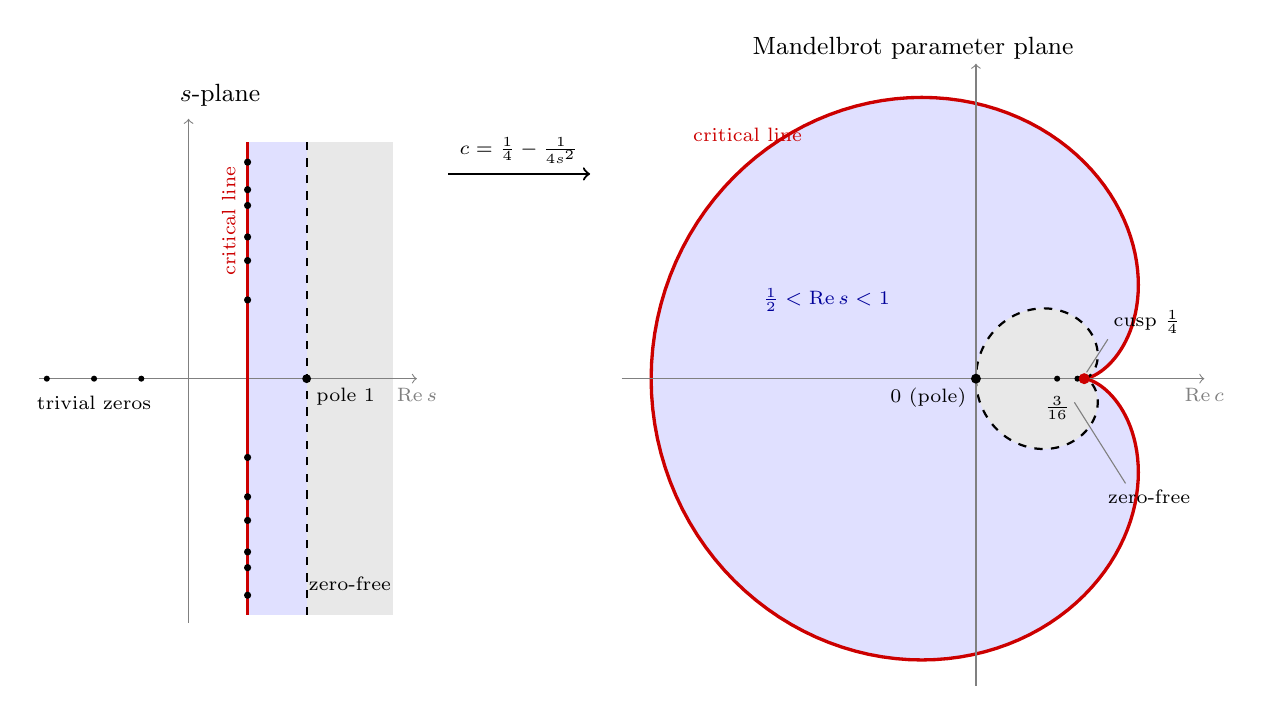
\begin{tikzpicture}
\begin{scope}[shift={(-8.3,0)}]
  \fill[blue!12] (0.75,-3) rectangle (1.5,3);
  \fill[gray!18] (1.5,-3) rectangle (2.6,3);
  \draw[->,gray] (-1.9,0)--(2.9,0) node[below]{\scriptsize$\operatorname{Re}s$};
  \draw[->,gray] (0,-3.1)--(0,3.3);
  \draw[very thick,red!80!black] (0.75,-3)--(0.75,3);
  \draw[thick,dashed] (1.5,-3)--(1.5,3);
  \node[red!80!black,rotate=90,anchor=south] at (0.72,2.0) {\scriptsize critical line};
  \fill (1.5,0) circle (1.6pt) node[below right]{\scriptsize pole $1$};
  \foreach \y in {1.0,1.5,1.8,2.2,2.4,2.75,-1.0,-1.5,-1.8,-2.2,-2.4,-2.75}
    \fill[black] (0.75,\y) circle (1.3pt);
  \foreach \x in {-0.6,-1.2,-1.8} \fill (\x,0) circle (1.1pt);
  \node[anchor=north] at (-1.2,-0.1) {\scriptsize trivial zeros};
  \node at (2.05,-2.6) {\scriptsize zero-free};
  \node at (0.4,3.6) {\small $s$-plane};
\end{scope}
\draw[->,thick] (-5.0,2.6) -- (-3.2,2.6) node[midway,above]{\scriptsize $c=\tfrac14-\tfrac1{4s^{2}}$};
\begin{scope}[shift={(1.7,0)}]
  \fill[blue!12] (1.3750,0.0000) -- (1.3767,0.0001) -- (1.3817,0.0005) -- (1.3900,0.0016) -- (1.4015,0.0037) -- (1.4161,0.0073) -- (1.4338,0.0125) -- (1.4543,0.0198) -- (1.4774,0.0294) -- (1.5030,0.0416) -- (1.5308,0.0567) -- (1.5607,0.0750) -- (1.5922,0.0967) -- (1.6251,0.1220) -- (1.6592,0.1511) -- (1.6941,0.1842) -- (1.7294,0.2214) -- (1.7648,0.2629) -- (1.7999,0.3087) -- (1.8344,0.3589) -- (1.8679,0.4136) -- (1.8999,0.4726) -- (1.9302,0.5361) -- (1.9583,0.6040) -- (1.9838,0.6762) -- (2.0064,0.7525) -- (2.0257,0.8329) -- (2.0413,0.9171) -- (2.0529,1.0050) -- (2.0600,1.0963) -- (2.0625,1.1908) -- (2.0599,1.2882) -- (2.0521,1.3882) -- (2.0386,1.4904) -- (2.0193,1.5946) -- (1.9939,1.7003) -- (1.9622,1.8072) -- (1.9241,1.9148) -- (1.8793,2.0228) -- (1.8279,2.1306) -- (1.7696,2.2379) -- (1.7045,2.3442) -- (1.6324,2.4491) -- (1.5534,2.5519) -- (1.4676,2.6524) -- (1.3750,2.7500) -- (1.2757,2.8442) -- (1.1698,2.9347) -- (1.0575,3.0208) -- (0.9390,3.1022) -- (0.8145,3.1785) -- (0.6844,3.2492) -- (0.5488,3.3138) -- (0.4081,3.3721) -- (0.2626,3.4236) -- (0.1128,3.4680) -- (-0.0411,3.5049) -- (-0.1985,3.5341) -- (-0.3590,3.5552) -- (-0.5222,3.5680) -- (-0.6875,3.5724) -- (-0.8545,3.5680) -- (-1.0227,3.5547) -- (-1.1915,3.5325) -- (-1.3604,3.5012) -- (-1.5289,3.4607) -- (-1.6964,3.4111) -- (-1.8623,3.3523) -- (-2.0262,3.2845) -- (-2.1874,3.2076) -- (-2.3454,3.1218) -- (-2.4997,3.0272) -- (-2.6497,2.9241) -- (-2.7949,2.8127) -- (-2.9349,2.6931) -- (-3.0691,2.5658) -- (-3.1970,2.4310) -- (-3.3182,2.2890) -- (-3.4323,2.1403) -- (-3.5388,1.9853) -- (-3.6375,1.8244) -- (-3.7278,1.6580) -- (-3.8095,1.4866) -- (-3.8824,1.3108) -- (-3.9460,1.1310) -- (-4.0003,0.9478) -- (-4.0450,0.7617) -- (-4.0799,0.5733) -- (-4.1049,0.3832) -- (-4.1200,0.1919) -- (-4.1250,0.0000) -- (-4.1200,-0.1919) -- (-4.1049,-0.3832) -- (-4.0799,-0.5733) -- (-4.0450,-0.7617) -- (-4.0003,-0.9478) -- (-3.9460,-1.1310) -- (-3.8824,-1.3108) -- (-3.8095,-1.4866) -- (-3.7278,-1.6580) -- (-3.6375,-1.8244) -- (-3.5388,-1.9853) -- (-3.4323,-2.1403) -- (-3.3182,-2.2890) -- (-3.1970,-2.4310) -- (-3.0691,-2.5658) -- (-2.9349,-2.6931) -- (-2.7949,-2.8127) -- (-2.6497,-2.9241) -- (-2.4997,-3.0272) -- (-2.3454,-3.1218) -- (-2.1874,-3.2076) -- (-2.0262,-3.2845) -- (-1.8623,-3.3523) -- (-1.6964,-3.4111) -- (-1.5289,-3.4607) -- (-1.3604,-3.5012) -- (-1.1915,-3.5325) -- (-1.0227,-3.5547) -- (-0.8545,-3.5680) -- (-0.6875,-3.5724) -- (-0.5222,-3.5680) -- (-0.3590,-3.5552) -- (-0.1985,-3.5341) -- (-0.0411,-3.5049) -- (0.1128,-3.4680) -- (0.2626,-3.4236) -- (0.4081,-3.3721) -- (0.5488,-3.3138) -- (0.6844,-3.2492) -- (0.8145,-3.1785) -- (0.9390,-3.1022) -- (1.0575,-3.0208) -- (1.1698,-2.9347) -- (1.2757,-2.8442) -- (1.3750,-2.7500) -- (1.4676,-2.6524) -- (1.5534,-2.5519) -- (1.6324,-2.4491) -- (1.7045,-2.3442) -- (1.7696,-2.2379) -- (1.8279,-2.1306) -- (1.8793,-2.0228) -- (1.9241,-1.9148) -- (1.9622,-1.8072) -- (1.9939,-1.7003) -- (2.0193,-1.5946) -- (2.0386,-1.4904) -- (2.0521,-1.3882) -- (2.0599,-1.2882) -- (2.0625,-1.1908) -- (2.0600,-1.0963) -- (2.0529,-1.0050) -- (2.0413,-0.9171) -- (2.0257,-0.8329) -- (2.0064,-0.7525) -- (1.9838,-0.6762) -- (1.9583,-0.6040) -- (1.9302,-0.5361) -- (1.8999,-0.4726) -- (1.8679,-0.4136) -- (1.8344,-0.3589) -- (1.7999,-0.3087) -- (1.7648,-0.2629) -- (1.7294,-0.2214) -- (1.6941,-0.1842) -- (1.6592,-0.1511) -- (1.6251,-0.1220) -- (1.5922,-0.0967) -- (1.5607,-0.0750) -- (1.5308,-0.0567) -- (1.5030,-0.0416) -- (1.4774,-0.0294) -- (1.4543,-0.0198) -- (1.4338,-0.0125) -- (1.4161,-0.0073) -- (1.4015,-0.0037) -- (1.3900,-0.0016) -- (1.3817,-0.0005) -- (1.3767,-0.0001) -- (1.3750,0.0000) -- cycle;
  \fill[gray!18] (1.3750,0.0000) -- (1.3754,0.0000) -- (1.3767,0.0001) -- (1.3787,0.0004) -- (1.3816,0.0009) -- (1.3853,0.0018) -- (1.3897,0.0031) -- (1.3948,0.0049) -- (1.4006,0.0073) -- (1.4070,0.0104) -- (1.4140,0.0142) -- (1.4214,0.0188) -- (1.4293,0.0242) -- (1.4375,0.0305) -- (1.4461,0.0378) -- (1.4548,0.0461) -- (1.4636,0.0554) -- (1.4724,0.0657) -- (1.4812,0.0772) -- (1.4898,0.0897) -- (1.4982,0.1034) -- (1.5062,0.1182) -- (1.5138,0.1340) -- (1.5208,0.1510) -- (1.5272,0.1690) -- (1.5329,0.1881) -- (1.5377,0.2082) -- (1.5416,0.2293) -- (1.5445,0.2512) -- (1.5463,0.2741) -- (1.5469,0.2977) -- (1.5462,0.3220) -- (1.5443,0.3470) -- (1.5409,0.3726) -- (1.5361,0.3987) -- (1.5297,0.4251) -- (1.5218,0.4518) -- (1.5123,0.4787) -- (1.5011,0.5057) -- (1.4882,0.5327) -- (1.4737,0.5595) -- (1.4574,0.5861) -- (1.4394,0.6123) -- (1.4196,0.6380) -- (1.3982,0.6631) -- (1.3750,0.6875) -- (1.3502,0.7111) -- (1.3237,0.7337) -- (1.2956,0.7552) -- (1.2660,0.7756) -- (1.2349,0.7946) -- (1.2023,0.8123) -- (1.1684,0.8285) -- (1.1333,0.8430) -- (1.0969,0.8559) -- (1.0594,0.8670) -- (1.0210,0.8762) -- (0.9816,0.8835) -- (0.9415,0.8888) -- (0.9007,0.8920) -- (0.8594,0.8931) -- (0.8176,0.8920) -- (0.7756,0.8887) -- (0.7334,0.8831) -- (0.6911,0.8753) -- (0.6490,0.8652) -- (0.6072,0.8528) -- (0.5657,0.8381) -- (0.5247,0.8211) -- (0.4844,0.8019) -- (0.4449,0.7804) -- (0.4063,0.7568) -- (0.3688,0.7310) -- (0.3325,0.7032) -- (0.2975,0.6733) -- (0.2640,0.6414) -- (0.2320,0.6077) -- (0.2017,0.5723) -- (0.1732,0.5351) -- (0.1465,0.4963) -- (0.1219,0.4561) -- (0.0993,0.4145) -- (0.0789,0.3717) -- (0.0607,0.3277) -- (0.0447,0.2828) -- (0.0312,0.2370) -- (0.0200,0.1904) -- (0.0113,0.1433) -- (0.0050,0.0958) -- (0.0013,0.0480) -- (0.0000,0.0000) -- (0.0013,-0.0480) -- (0.0050,-0.0958) -- (0.0113,-0.1433) -- (0.0200,-0.1904) -- (0.0312,-0.2370) -- (0.0447,-0.2828) -- (0.0607,-0.3277) -- (0.0789,-0.3717) -- (0.0993,-0.4145) -- (0.1219,-0.4561) -- (0.1465,-0.4963) -- (0.1732,-0.5351) -- (0.2017,-0.5723) -- (0.2320,-0.6077) -- (0.2640,-0.6414) -- (0.2975,-0.6733) -- (0.3325,-0.7032) -- (0.3688,-0.7310) -- (0.4063,-0.7568) -- (0.4449,-0.7804) -- (0.4844,-0.8019) -- (0.5247,-0.8211) -- (0.5657,-0.8381) -- (0.6072,-0.8528) -- (0.6490,-0.8652) -- (0.6911,-0.8753) -- (0.7334,-0.8831) -- (0.7756,-0.8887) -- (0.8176,-0.8920) -- (0.8594,-0.8931) -- (0.9007,-0.8920) -- (0.9415,-0.8888) -- (0.9816,-0.8835) -- (1.0210,-0.8762) -- (1.0594,-0.8670) -- (1.0969,-0.8559) -- (1.1333,-0.8430) -- (1.1684,-0.8285) -- (1.2023,-0.8123) -- (1.2349,-0.7946) -- (1.2660,-0.7756) -- (1.2956,-0.7552) -- (1.3237,-0.7337) -- (1.3502,-0.7111) -- (1.3750,-0.6875) -- (1.3982,-0.6631) -- (1.4196,-0.6380) -- (1.4394,-0.6123) -- (1.4574,-0.5861) -- (1.4737,-0.5595) -- (1.4882,-0.5327) -- (1.5011,-0.5057) -- (1.5123,-0.4787) -- (1.5218,-0.4518) -- (1.5297,-0.4251) -- (1.5361,-0.3987) -- (1.5409,-0.3726) -- (1.5443,-0.3470) -- (1.5462,-0.3220) -- (1.5469,-0.2977) -- (1.5463,-0.2741) -- (1.5445,-0.2512) -- (1.5416,-0.2293) -- (1.5377,-0.2082) -- (1.5329,-0.1881) -- (1.5272,-0.1690) -- (1.5208,-0.1510) -- (1.5138,-0.1340) -- (1.5062,-0.1182) -- (1.4982,-0.1034) -- (1.4898,-0.0897) -- (1.4812,-0.0772) -- (1.4724,-0.0657) -- (1.4636,-0.0554) -- (1.4548,-0.0461) -- (1.4461,-0.0378) -- (1.4375,-0.0305) -- (1.4293,-0.0242) -- (1.4214,-0.0188) -- (1.4140,-0.0142) -- (1.4070,-0.0104) -- (1.4006,-0.0073) -- (1.3948,-0.0049) -- (1.3897,-0.0031) -- (1.3853,-0.0018) -- (1.3816,-0.0009) -- (1.3787,-0.0004) -- (1.3767,-0.0001) -- (1.3754,-0.0000) -- (1.3750,0.0000) -- cycle;
  \draw[very thick,red!80!black] (1.3750,0.0000) -- (1.3767,0.0001) -- (1.3817,0.0005) -- (1.3900,0.0016) -- (1.4015,0.0037) -- (1.4161,0.0073) -- (1.4338,0.0125) -- (1.4543,0.0198) -- (1.4774,0.0294) -- (1.5030,0.0416) -- (1.5308,0.0567) -- (1.5607,0.0750) -- (1.5922,0.0967) -- (1.6251,0.1220) -- (1.6592,0.1511) -- (1.6941,0.1842) -- (1.7294,0.2214) -- (1.7648,0.2629) -- (1.7999,0.3087) -- (1.8344,0.3589) -- (1.8679,0.4136) -- (1.8999,0.4726) -- (1.9302,0.5361) -- (1.9583,0.6040) -- (1.9838,0.6762) -- (2.0064,0.7525) -- (2.0257,0.8329) -- (2.0413,0.9171) -- (2.0529,1.0050) -- (2.0600,1.0963) -- (2.0625,1.1908) -- (2.0599,1.2882) -- (2.0521,1.3882) -- (2.0386,1.4904) -- (2.0193,1.5946) -- (1.9939,1.7003) -- (1.9622,1.8072) -- (1.9241,1.9148) -- (1.8793,2.0228) -- (1.8279,2.1306) -- (1.7696,2.2379) -- (1.7045,2.3442) -- (1.6324,2.4491) -- (1.5534,2.5519) -- (1.4676,2.6524) -- (1.3750,2.7500) -- (1.2757,2.8442) -- (1.1698,2.9347) -- (1.0575,3.0208) -- (0.9390,3.1022) -- (0.8145,3.1785) -- (0.6844,3.2492) -- (0.5488,3.3138) -- (0.4081,3.3721) -- (0.2626,3.4236) -- (0.1128,3.4680) -- (-0.0411,3.5049) -- (-0.1985,3.5341) -- (-0.3590,3.5552) -- (-0.5222,3.5680) -- (-0.6875,3.5724) -- (-0.8545,3.5680) -- (-1.0227,3.5547) -- (-1.1915,3.5325) -- (-1.3604,3.5012) -- (-1.5289,3.4607) -- (-1.6964,3.4111) -- (-1.8623,3.3523) -- (-2.0262,3.2845) -- (-2.1874,3.2076) -- (-2.3454,3.1218) -- (-2.4997,3.0272) -- (-2.6497,2.9241) -- (-2.7949,2.8127) -- (-2.9349,2.6931) -- (-3.0691,2.5658) -- (-3.1970,2.4310) -- (-3.3182,2.2890) -- (-3.4323,2.1403) -- (-3.5388,1.9853) -- (-3.6375,1.8244) -- (-3.7278,1.6580) -- (-3.8095,1.4866) -- (-3.8824,1.3108) -- (-3.9460,1.1310) -- (-4.0003,0.9478) -- (-4.0450,0.7617) -- (-4.0799,0.5733) -- (-4.1049,0.3832) -- (-4.1200,0.1919) -- (-4.1250,0.0000) -- (-4.1200,-0.1919) -- (-4.1049,-0.3832) -- (-4.0799,-0.5733) -- (-4.0450,-0.7617) -- (-4.0003,-0.9478) -- (-3.9460,-1.1310) -- (-3.8824,-1.3108) -- (-3.8095,-1.4866) -- (-3.7278,-1.6580) -- (-3.6375,-1.8244) -- (-3.5388,-1.9853) -- (-3.4323,-2.1403) -- (-3.3182,-2.2890) -- (-3.1970,-2.4310) -- (-3.0691,-2.5658) -- (-2.9349,-2.6931) -- (-2.7949,-2.8127) -- (-2.6497,-2.9241) -- (-2.4997,-3.0272) -- (-2.3454,-3.1218) -- (-2.1874,-3.2076) -- (-2.0262,-3.2845) -- (-1.8623,-3.3523) -- (-1.6964,-3.4111) -- (-1.5289,-3.4607) -- (-1.3604,-3.5012) -- (-1.1915,-3.5325) -- (-1.0227,-3.5547) -- (-0.8545,-3.5680) -- (-0.6875,-3.5724) -- (-0.5222,-3.5680) -- (-0.3590,-3.5552) -- (-0.1985,-3.5341) -- (-0.0411,-3.5049) -- (0.1128,-3.4680) -- (0.2626,-3.4236) -- (0.4081,-3.3721) -- (0.5488,-3.3138) -- (0.6844,-3.2492) -- (0.8145,-3.1785) -- (0.9390,-3.1022) -- (1.0575,-3.0208) -- (1.1698,-2.9347) -- (1.2757,-2.8442) -- (1.3750,-2.7500) -- (1.4676,-2.6524) -- (1.5534,-2.5519) -- (1.6324,-2.4491) -- (1.7045,-2.3442) -- (1.7696,-2.2379) -- (1.8279,-2.1306) -- (1.8793,-2.0228) -- (1.9241,-1.9148) -- (1.9622,-1.8072) -- (1.9939,-1.7003) -- (2.0193,-1.5946) -- (2.0386,-1.4904) -- (2.0521,-1.3882) -- (2.0599,-1.2882) -- (2.0625,-1.1908) -- (2.0600,-1.0963) -- (2.0529,-1.0050) -- (2.0413,-0.9171) -- (2.0257,-0.8329) -- (2.0064,-0.7525) -- (1.9838,-0.6762) -- (1.9583,-0.6040) -- (1.9302,-0.5361) -- (1.8999,-0.4726) -- (1.8679,-0.4136) -- (1.8344,-0.3589) -- (1.7999,-0.3087) -- (1.7648,-0.2629) -- (1.7294,-0.2214) -- (1.6941,-0.1842) -- (1.6592,-0.1511) -- (1.6251,-0.1220) -- (1.5922,-0.0967) -- (1.5607,-0.0750) -- (1.5308,-0.0567) -- (1.5030,-0.0416) -- (1.4774,-0.0294) -- (1.4543,-0.0198) -- (1.4338,-0.0125) -- (1.4161,-0.0073) -- (1.4015,-0.0037) -- (1.3900,-0.0016) -- (1.3817,-0.0005) -- (1.3767,-0.0001) -- (1.3750,0.0000) -- cycle;
  \draw[thick,dashed] (1.3750,0.0000) -- (1.3754,0.0000) -- (1.3767,0.0001) -- (1.3787,0.0004) -- (1.3816,0.0009) -- (1.3853,0.0018) -- (1.3897,0.0031) -- (1.3948,0.0049) -- (1.4006,0.0073) -- (1.4070,0.0104) -- (1.4140,0.0142) -- (1.4214,0.0188) -- (1.4293,0.0242) -- (1.4375,0.0305) -- (1.4461,0.0378) -- (1.4548,0.0461) -- (1.4636,0.0554) -- (1.4724,0.0657) -- (1.4812,0.0772) -- (1.4898,0.0897) -- (1.4982,0.1034) -- (1.5062,0.1182) -- (1.5138,0.1340) -- (1.5208,0.1510) -- (1.5272,0.1690) -- (1.5329,0.1881) -- (1.5377,0.2082) -- (1.5416,0.2293) -- (1.5445,0.2512) -- (1.5463,0.2741) -- (1.5469,0.2977) -- (1.5462,0.3220) -- (1.5443,0.3470) -- (1.5409,0.3726) -- (1.5361,0.3987) -- (1.5297,0.4251) -- (1.5218,0.4518) -- (1.5123,0.4787) -- (1.5011,0.5057) -- (1.4882,0.5327) -- (1.4737,0.5595) -- (1.4574,0.5861) -- (1.4394,0.6123) -- (1.4196,0.6380) -- (1.3982,0.6631) -- (1.3750,0.6875) -- (1.3502,0.7111) -- (1.3237,0.7337) -- (1.2956,0.7552) -- (1.2660,0.7756) -- (1.2349,0.7946) -- (1.2023,0.8123) -- (1.1684,0.8285) -- (1.1333,0.8430) -- (1.0969,0.8559) -- (1.0594,0.8670) -- (1.0210,0.8762) -- (0.9816,0.8835) -- (0.9415,0.8888) -- (0.9007,0.8920) -- (0.8594,0.8931) -- (0.8176,0.8920) -- (0.7756,0.8887) -- (0.7334,0.8831) -- (0.6911,0.8753) -- (0.6490,0.8652) -- (0.6072,0.8528) -- (0.5657,0.8381) -- (0.5247,0.8211) -- (0.4844,0.8019) -- (0.4449,0.7804) -- (0.4063,0.7568) -- (0.3688,0.7310) -- (0.3325,0.7032) -- (0.2975,0.6733) -- (0.2640,0.6414) -- (0.2320,0.6077) -- (0.2017,0.5723) -- (0.1732,0.5351) -- (0.1465,0.4963) -- (0.1219,0.4561) -- (0.0993,0.4145) -- (0.0789,0.3717) -- (0.0607,0.3277) -- (0.0447,0.2828) -- (0.0312,0.2370) -- (0.0200,0.1904) -- (0.0113,0.1433) -- (0.0050,0.0958) -- (0.0013,0.0480) -- (0.0000,0.0000) -- (0.0013,-0.0480) -- (0.0050,-0.0958) -- (0.0113,-0.1433) -- (0.0200,-0.1904) -- (0.0312,-0.2370) -- (0.0447,-0.2828) -- (0.0607,-0.3277) -- (0.0789,-0.3717) -- (0.0993,-0.4145) -- (0.1219,-0.4561) -- (0.1465,-0.4963) -- (0.1732,-0.5351) -- (0.2017,-0.5723) -- (0.2320,-0.6077) -- (0.2640,-0.6414) -- (0.2975,-0.6733) -- (0.3325,-0.7032) -- (0.3688,-0.7310) -- (0.4063,-0.7568) -- (0.4449,-0.7804) -- (0.4844,-0.8019) -- (0.5247,-0.8211) -- (0.5657,-0.8381) -- (0.6072,-0.8528) -- (0.6490,-0.8652) -- (0.6911,-0.8753) -- (0.7334,-0.8831) -- (0.7756,-0.8887) -- (0.8176,-0.8920) -- (0.8594,-0.8931) -- (0.9007,-0.8920) -- (0.9415,-0.8888) -- (0.9816,-0.8835) -- (1.0210,-0.8762) -- (1.0594,-0.8670) -- (1.0969,-0.8559) -- (1.1333,-0.8430) -- (1.1684,-0.8285) -- (1.2023,-0.8123) -- (1.2349,-0.7946) -- (1.2660,-0.7756) -- (1.2956,-0.7552) -- (1.3237,-0.7337) -- (1.3502,-0.7111) -- (1.3750,-0.6875) -- (1.3982,-0.6631) -- (1.4196,-0.6380) -- (1.4394,-0.6123) -- (1.4574,-0.5861) -- (1.4737,-0.5595) -- (1.4882,-0.5327) -- (1.5011,-0.5057) -- (1.5123,-0.4787) -- (1.5218,-0.4518) -- (1.5297,-0.4251) -- (1.5361,-0.3987) -- (1.5409,-0.3726) -- (1.5443,-0.3470) -- (1.5462,-0.3220) -- (1.5469,-0.2977) -- (1.5463,-0.2741) -- (1.5445,-0.2512) -- (1.5416,-0.2293) -- (1.5377,-0.2082) -- (1.5329,-0.1881) -- (1.5272,-0.1690) -- (1.5208,-0.1510) -- (1.5138,-0.1340) -- (1.5062,-0.1182) -- (1.4982,-0.1034) -- (1.4898,-0.0897) -- (1.4812,-0.0772) -- (1.4724,-0.0657) -- (1.4636,-0.0554) -- (1.4548,-0.0461) -- (1.4461,-0.0378) -- (1.4375,-0.0305) -- (1.4293,-0.0242) -- (1.4214,-0.0188) -- (1.4140,-0.0142) -- (1.4070,-0.0104) -- (1.4006,-0.0073) -- (1.3948,-0.0049) -- (1.3897,-0.0031) -- (1.3853,-0.0018) -- (1.3816,-0.0009) -- (1.3787,-0.0004) -- (1.3767,-0.0001) -- (1.3754,-0.0000) -- (1.3750,0.0000) -- cycle;
  \draw[->,gray] (-4.5,0)--(2.9,0) node[below]{\scriptsize$\operatorname{Re}c$};
  \draw[->,gray] (0,-3.9)--(0,4.0);
  \fill (0,0) circle (1.8pt) node[below left]{\scriptsize $0$ (pole)};
  \fill[black] (1.0312,0) circle (1.1pt);
  \fill[black] (1.2891,0) circle (1.1pt);
  \fill[black] (1.3368,0) circle (1.1pt);
  \fill[black] (1.3535,0) circle (1.1pt);
  \fill[black] (1.3613,0) circle (1.1pt);
  \fill[black] (1.3655,0) circle (1.1pt);
  \node[anchor=north] at (1.0312,-0.1) {\scriptsize $\tfrac3{16}$};
  \fill[red!80!black] (1.3750,0) circle (2pt);
  \node[anchor=south west] at (1.6250,0.45) {\scriptsize cusp $\tfrac14$};
  \draw[gray] (1.6750,0.5)--(1.4050,0.08);
  \node[red!80!black] at (-2.9,3.1) {\scriptsize critical line};
  \node[blue!60!black] at (-1.9,1.0) {\scriptsize $\tfrac12<\operatorname{Re}s<1$};
  \node at (2.2,-1.5) {\scriptsize zero-free};
  \draw[gray] (1.9,-1.33)--(1.25,-0.3);
  \node at (-0.8,4.2) {\small Mandelbrot parameter plane};
\end{scope}
\end{tikzpicture}

\small The dictionary. Red: the critical line and its image, the boundary of the main
cardioid. Blue: the right half of the critical strip and its image, a crescent. Grey:
the classical zero-free region $\Re s\ge1$ and its image, the quarter-size cardioid.
Dots on the real axis: the trivial zeros, marching into the cusp from inside.
The nontrivial zeros lie on the red rim and accumulate at the cusp (the $s$-plane
picture is schematic).
\end{center}

\section{A finite Li criterion}
Li's criterion says that the Riemann hypothesis is equivalent to
$\lambda_n=\sum_\rho\bigl[1-(1-\tfrac1\rho)^{n}\bigr]\ge0$ for all $n\ge1$, the sum
running over all nontrivial zeros. Bombieri and Lagarias showed that this is a
general fact about multisets of complex numbers. In the dictionary, $1-\tfrac1\rho$
is the multiplier $\mu_\rho$ of the fixed point, and $\mu_\rho^{\,n}$ is the multiplier
of the same fixed point for the $n$-th iterate of $f_{c(\rho)}$.

\begin{theorem}[Finite Bombieri--Lagarias]\label{fli}
Let $\mu_1,\dots,\mu_k$ be complex numbers (repetitions allowed). Then
\[
  \sum_{j=1}^{k}\Re\bigl(1-\mu_j^{\,n}\bigr)\ge0\ \text{ for all } n\ge1
  \quad\Longleftrightarrow\quad |\mu_j|\le1\ \text{ for all } j .
\]
\end{theorem}

\begin{proof}[Proof sketch]
If all $|\mu_j|\le1$ then each term is at least $1-|\mu_j|^{n}\ge0$. Conversely suppose
$|\mu_{j_0}|=r>1$. Write $\mu_j=|\mu_j|\,w_j$ with $|w_j|=1$. The sequence
$n\mapsto(w_1^{\,n},\dots,w_k^{\,n})$ lives in a compact set, so it has a convergent
subsequence; taking differences of two far-apart indices gives arbitrarily large $n$
with $|w_j^{\,n}-1|<\tfrac12$ for all $j$ at once. For such $n$,
$\Re\mu_j^{\,n}\ge\tfrac12|\mu_j|^{n}\ge0$ for every $j$, so
$\sum_j\Re(1-\mu_j^{\,n})\le k-\tfrac12r^{n}$, which is negative once $r^{n}>2k$.
\end{proof}

\begin{corollary}\label{half}
For nonzero $s_1,\dots,s_k$:\quad
$\sum_j\Re\bigl(1-(1-\tfrac1{s_j})^{n}\bigr)\ge0$ for all $n\ge1$ if and only if
$\Re s_j\ge\tfrac12$ for all $j$.
\end{corollary}

\begin{theorem}[Riemann hypothesis via finite Li sums]\label{rhli}
The Riemann hypothesis holds if and only if for every finite set $Z$ of nontrivial
zeros of $\zeta$ and every $n\ge1$,
\[
  \sum_{\rho\in Z}\Re\Bigl(1-\bigl(1-\tfrac1\rho\bigr)^{n}\Bigr)\ \ge\ 0 .
\]
\end{theorem}

The proof applies Corollary~\ref{half} to $\{\rho\}$ and to $\{1-\rho\}$, using that
nontrivial zeros come in pairs $\rho,1-\rho$ (functional equation). Unlike Li's
criterion, no infinite sum over zeros is needed, which is what makes the statement
easy to formalise; the price is that the hypothesis quantifies over all finite sets. Taking $Z=\{\rho\}$ gives the termwise form: the Riemann hypothesis holds if and only if
$\Re\bigl((1-\tfrac1\rho)^{n}\bigr)\le1$ for every nontrivial zero $\rho$ and every $n\ge1$, because a
complex number has all its powers in the half-plane $\Re z\le1$ exactly when it lies in the closed
unit disc.

\section{What is new and what is not}
\begin{itemize}[leftmargin=1.4em]
\item The link between the Riemann hypothesis and the holomorphic index is due to
Kawahira (\emph{The Riemann hypothesis and holomorphic index in complex dynamics},
arXiv:1602.06843), who shows that RH with simple
zeros is equivalent to a certain meromorphic map having no attracting fixed point.
Item~(d) of Theorem~\ref{rh} is in the same spirit and is also the classical unit-disc
form of RH that underlies Li's criterion.
\item That the main cardioid is $\{\mu/2-\mu^{2}/4:|\mu|<1\}$, and the index
trichotomy, are textbook complex dynamics (Milnor, \emph{Dynamics in One Complex
Variable}).
\item Theorem~\ref{fli} is the finite case of Theorem~1 of Bombieri and Lagarias
(\emph{Complements to Li's criterion for the Riemann hypothesis}, J.\ Number Theory 77
(1999)), up to the substitution $\rho\mapsto1-\rho$; the simultaneous-approximation
argument is the standard one.
\item We could not find the Mandelbrot form (b), (c), the quarter-cardioid picture of the
zero-free region, or Theorem~\ref{rhli} stated anywhere, and we could not find a Lean
formalisation of any of the above. Both searches were short.
\end{itemize}

\section{Formalisation}
Everything above is proved in Lean~4 against Mathlib, with no \texttt{sorry} and only
the axioms \texttt{propext}, \texttt{Classical.choice}, \texttt{Quot.sound}. The
equivalences are with Mathlib's own \texttt{RiemannHypothesis}; the proof of RH itself
is not imported.

\begin{itemize}[leftmargin=1.4em,itemsep=1pt]\small\raggedright
\item Theorem~\ref{dict}: \texttt{dictionary}, \texttt{attracting\_cardioidParam\_iff}, \texttt{neutral\_cardioidParam\_iff}, \texttt{cardioidParam\_one}, \texttt{cardioidParam\_trivial\_zero}, \texttt{attracting\_scaled\_iff}.
\item Theorem~\ref{rh}: \texttt{riemannHypothesis\_iff\_no\_zero\_inside\_cardioid}, \texttt{riemannHypothesis\_iff\_neutral}, \texttt{riemannHypothesis\_iff\_zero\_free\_at\_attracting\_index}.
\item Proposition~\ref{quarter}: \texttt{no\_zero\_in\_quarter\_cardioid}.
\item Theorem~\ref{fli} and Corollary~\ref{half}: \texttt{finite\_li\_criterion}, \texttt{finite\_li\_criterion\_half\_plane}.
\item Theorem~\ref{rhli}: \texttt{riemannHypothesis\_iff\_finite\_li\_sums\_nonneg}.
\end{itemize}

\medskip\noindent
Both files, \texttt{Slopollary3.lean} and \texttt{FiniteLi.lean}, compile exactly as distributed on \texttt{live.lean-lang.org} (Lean 4.37.0-rc1 with current Mathlib, 26 November 2026), with no errors. \texttt{FiniteLi.lean} gives one deprecation warning.
\end{document}
